\documentclass[main.tex]{subfiles}
\begin{document}\newpage
\setdoublesep{0.35700 em}  % 'Bond Spacing'
\setatomsep{1.78500 em}    % 'Fixed Length'
\setbondoffset{0.18265 em} % 'Margin Width'
\newcommand{\bondwidth}{0.06642 em} % 'Line Width'
\setbondstyle{line width = \bondwidth}
\newgeometry{left=0.8in,right=0.8in, top=2.5cm,bottom=2cm}
\fancyhfoffset[E,O]{0pt}
\setlength{\columnsep}{30pt}
\begin{conclusion}
\end{conclusion}
%\setstretch{0.3}
\begin{multicols*}{2}\setcounter{numA}{1}

{\raggedright\textsc{\textbf{Gases And Its Properties }}\par}

%%%%%PROBLEM
\begin{question}[ID=\the\value{numA}]\SetQuestionProperties{section-title=\nameref{sec:units}}
Convert the following properties:
\begin{inparaenum}[(a)]	
\item  A pressure value of 2 atm into mmHg
%\item  A pressure value of 900 mmHg into torr
\item  A pressure value of 3000 Pa into atm
\item  A temperature value of 25$^{\circ}$C into K
%\item  A temperature value of 400K into $^{\circ}$C
\end{inparaenum} 
\end{question}
\begin{solution}
\begin{inparaenum}[(a)]	
\item  1520 mmHg
%\item  $7\times 10^{5}$ torr
\item $2.96\times 10^{-2}$ atm
\item 298K
%\item 121$^{\circ}$C
\end{inparaenum} 
\hspace{0.1cm}\end{solution}\stepcounter{numA}%%%%%%%%%%%%
%%%%%PROBLEM
\begin{question}[ID=\the\value{numA}]\SetQuestionProperties{section-title=\nameref{sec:units}}
Convert the following properties:
\begin{inparaenum}[(a)]	
\item  A pressure value of 900 mmHg into torr
\item  A temperature value of 400K into $^{\circ}$C
\end{inparaenum} 
\end{question}
\begin{solution}
\begin{inparaenum}[(a)]	
\item  $7\times 10^{5}$ torr
\item 121$^{\circ}$C
\end{inparaenum} 
\hspace{0.1cm}\end{solution}\stepcounter{numA}%%%%%%%%%%%%




%%%%%PROBLEM
\begin{question}[ID=\the\value{numA}]\SetQuestionProperties{section-title=\nameref{sec:units}}
An open-tube manometer is used to measure the pressure of a given gas. When there is no gas in the container, the mercury levels are equal in both sides of the u-tube.
%%%%%%%%%%MANOMETER
\begin{center}\begin{tikzpicture}[thick,scale=0.9, every node/.style={transform shape}]
\tikzset{edge/.style = {->,> = latex'}}
\def\r{1.1}% Mid-tube radius
\def\t{.2} % Tube thickness
\def\h{5}  % Straight height (total height is \r + \t/2 + \h)
\def\lh{2} % Left height
\def\rh{4} % Right height

\begin{scope}[xshift = 0cm]
\path [pattern=north west lines, pattern color=green]
  (-\r+\t/2, \lh) -- ++(0, -\lh) arc (180:360:\r-\t/2) |-
  ( \r+\t/2, \rh) -- ++(0, -\rh) arc (360:180:\r+\t/2) |- cycle;
\draw (-\r-\t/2, \lh-0.02) -- ++(\t,0)	 (\r-\t/2, \rh) -- ++(\t,0); 
\draw [black, thick] 
  (-\r-\t/2, \h) -- ++        (0, -\h) arc (180:360:\r+\t/2) -- ++(0, \h)
  (-\r+\t/2, \h) -- ++    (0, -\h) arc (180:360:\r-\t/2) -- ++(0, \h);
\draw [white, thick, fill=red!10] 
(-\r-\t/2+.1, \h     -1) -- ++ (-\r-2*\t/2, \h-0.1*\h-0.14cm) arc (0:350:1.0) -- ++ (\r+2*\t/2, \h-0.1*\h-0.16cm) |- cycle ;

 \draw[red!10,  fill=red!10]  (-\r-\t/2, 2.5*\lh) -- ++(\t-0.02,0) -- ++(0, -1.5*\lh) -- ++(-\t+0.04,0)  |- cycle ;
  \draw[black, thick]  (-\r-\t/2, 2.5*\lh-0.01) -- ++(\t,0)  ;
 % \draw[black, thick]  (\r-\t/2, \rh+1.0) -- ++(\t,0)  ;  % Open close
\node [shift={(1.2,5.2)}, font=\small,scale=0.7] {760mmHg};% Open close

\node [shift={(-3.5,4.1)}] {Gas};

\draw[<->] (-0,2) -- (-0,4) ;
\draw[dash pattern=on \pgflinewidth off 2pt] (-0,2) -- (-.9,2)   (-0,4) -- (.9,4);

\node [shift={(0.5,3.1)}] {\small 200mm};
\draw[thin] (1,4.5) -- ++(-.3,0) node [left,fill=white,font=\small,scale=0.7] {atmosphere};
\end{scope}

%\def\lh{2} % Left height
%\def\rh{1} % Right height
%\begin{scope}[xshift = 6cm]
%\path [pattern=north west lines, pattern color=green]
%  (-\r+\t/2, \lh) -- ++(0, -\lh) arc (180:360:\r-\t/2) |-
%  ( \r+\t/2, \rh) -- ++(0, -\rh) arc (360:180:\r+\t/2) |- cycle;
%\draw (-\r-\t/2, \lh-0.02) -- ++(\t,0)	 (\r-\t/2, \rh) -- ++(\t,0); 
%%\draw [black, thick] 
%%  (-\r-\t/2, \h) -- ++(0, -\h) arc (180:360:\r+\t/2) -- ++(0, \h)
%%  (-\r+\t/2, \h) -- ++(0, -\h) arc (180:360:\r-\t/2) -- ++(0, \h);
%\draw [black, thick] 
%  (-\r-\t/2, \h) -- ++        (0, -\h) arc (180:360:\r+\t/2) -- ++(0, \h)
%  (-\r+\t/2, \h) -- ++    (0, -\h) arc (180:360:\r-\t/2) -- ++(0, \h);
%\draw [white, thick, fill=red!10] 
%(-\r-\t/2+.1, \h     -1) -- ++ (-\r-2*\t/2, \h-0.1*\h-0.14cm) arc (0:350:1.0) -- ++ (\r+2*\t/2, \h-0.1*\h-0.16cm) |- cycle ;
%
% \draw[red!10,  fill=red!10]  (-\r-\t/2, 2.5*\lh) -- ++(\t-0.02,0) -- ++(0, -1.5*\lh) -- ++(-\t+0.04,0)  |- cycle ;
%  \draw[black, thick]  (-\r-\t/2, 2.5*\lh-0.01) -- ++(\t,0)  ;
% % \draw[black, thick]  (\r-\t/2, \rh+1.0) -- ++(\t,0)  ;  % Open close
%\node [shift={(1.2,5.2)}, font=\small,scale=0.5] {760mmHg};% Open close
%
%\node [shift={(-3.5,4.1)}] {Gas};
%
%\draw[<->] (-0,2) -- (-0,1) ;
%\draw[dash pattern=on \pgflinewidth off 2pt] (-0,2) -- (-.9,2)   (-0,1) -- (.9,1);
%
%\node [shift={(0.5,1.5)}] {\small   300mm};
%%\node [shift={(0.2,-1.8)}] {\small $\text{P}^{open}=\Delta \text{h}\text{dg}+\text{P}_{atm}$};
%\draw[thin] (1,4.5) -- ++(-.3,0) node [left,fill=white,font=\small,scale=0.7] {atmosphere};
%\end{scope}


\end{tikzpicture}\end{center}
%%%%%%%%%%MANOMETER

\begin{inparaenum}[(a)]	
\item  Would the gas pressure be lower or higher than the atmospheric pressure?
\item  Calculate the gas pressure in MPa.
\item  Calculate the gas pressure in Torr.
\end{inparaenum} 
\end{question}
\begin{solution}
\begin{inparaenum}[(a)]	
\item  higher 
\item  0.127MPa
\item  960mmHg
\end{inparaenum} 
\hspace{0.1cm}\end{solution}\stepcounter{numA}%%%%%%%%%%%%

%%%%%PROBLEM
\begin{question}[ID=\the\value{numA}]\SetQuestionProperties{section-title=\nameref{sec:units}}
An open-tube manometer is used to measure the pressure of a given gas. When there is no gas in the container, the mercury levels are equal in both sides of the u-tube.
%%%%%%%%%%MANOMETER
\begin{center}\begin{tikzpicture}[thick,scale=0.9, every node/.style={transform shape}]
\tikzset{edge/.style = {->,> = latex'}}
\def\r{1.1}% Mid-tube radius
\def\t{.2} % Tube thickness
\def\h{5}  % Straight height (total height is \r + \t/2 + \h)
\def\lh{2} % Left height
\def\rh{4} % Right height

%\begin{scope}[xshift = 0cm]
%\path [pattern=north west lines, pattern color=green]
%  (-\r+\t/2, \lh) -- ++(0, -\lh) arc (180:360:\r-\t/2) |-
%  ( \r+\t/2, \rh) -- ++(0, -\rh) arc (360:180:\r+\t/2) |- cycle;
%\draw (-\r-\t/2, \lh-0.02) -- ++(\t,0)	 (\r-\t/2, \rh) -- ++(\t,0); 
%\draw [black, thick] 
%  (-\r-\t/2, \h) -- ++        (0, -\h) arc (180:360:\r+\t/2) -- ++(0, \h)
%  (-\r+\t/2, \h) -- ++    (0, -\h) arc (180:360:\r-\t/2) -- ++(0, \h);
%\draw [white, thick, fill=red!10] 
%(-\r-\t/2+.1, \h     -1) -- ++ (-\r-2*\t/2, \h-0.1*\h-0.14cm) arc (0:350:1.0) -- ++ (\r+2*\t/2, \h-0.1*\h-0.16cm) |- cycle ;
%
% \draw[red!10,  fill=red!10]  (-\r-\t/2, 2.5*\lh) -- ++(\t-0.02,0) -- ++(0, -1.5*\lh) -- ++(-\t+0.04,0)  |- cycle ;
%  \draw[black, thick]  (-\r-\t/2, 2.5*\lh-0.01) -- ++(\t,0)  ;
% % \draw[black, thick]  (\r-\t/2, \rh+1.0) -- ++(\t,0)  ;  % Open close
%\node [shift={(1.2,5.2)}, font=\small,scale=0.7] {760mmHg};% Open close
%
%\node [shift={(-3.5,4.1)}] {Gas};
%
%\draw[<->] (-0,2) -- (-0,4) ;
%\draw[dash pattern=on \pgflinewidth off 2pt] (-0,2) -- (-.9,2)   (-0,4) -- (.9,4);
%
%\node [shift={(0.5,3.1)}] {\small 200mm};
%\draw[thin] (1,4.5) -- ++(-.3,0) node [left,fill=white,font=\small,scale=0.7] {atmosphere};
%\end{scope}

\def\lh{2} % Left height
\def\rh{1} % Right height
\begin{scope}[xshift = 6cm]
\path [pattern=north west lines, pattern color=green]
  (-\r+\t/2, \lh) -- ++(0, -\lh) arc (180:360:\r-\t/2) |-
  ( \r+\t/2, \rh) -- ++(0, -\rh) arc (360:180:\r+\t/2) |- cycle;
\draw (-\r-\t/2, \lh-0.02) -- ++(\t,0)	 (\r-\t/2, \rh) -- ++(\t,0); 
%\draw [black, thick] 
%  (-\r-\t/2, \h) -- ++(0, -\h) arc (180:360:\r+\t/2) -- ++(0, \h)
%  (-\r+\t/2, \h) -- ++(0, -\h) arc (180:360:\r-\t/2) -- ++(0, \h);
\draw [black, thick] 
  (-\r-\t/2, \h) -- ++        (0, -\h) arc (180:360:\r+\t/2) -- ++(0, \h)
  (-\r+\t/2, \h) -- ++    (0, -\h) arc (180:360:\r-\t/2) -- ++(0, \h);
\draw [white, thick, fill=red!10] 
(-\r-\t/2+.1, \h     -1) -- ++ (-\r-2*\t/2, \h-0.1*\h-0.14cm) arc (0:350:1.0) -- ++ (\r+2*\t/2, \h-0.1*\h-0.16cm) |- cycle ;

 \draw[red!10,  fill=red!10]  (-\r-\t/2, 2.5*\lh) -- ++(\t-0.02,0) -- ++(0, -1.5*\lh) -- ++(-\t+0.04,0)  |- cycle ;
  \draw[black, thick]  (-\r-\t/2, 2.5*\lh-0.01) -- ++(\t,0)  ;
 % \draw[black, thick]  (\r-\t/2, \rh+1.0) -- ++(\t,0)  ;  % Open close
\node [shift={(1.2,5.2)}, font=\small,scale=0.5] {760mmHg};% Open close

\node [shift={(-3.5,4.1)}] {Gas};

\draw[<->] (-0,2) -- (-0,1) ;
\draw[dash pattern=on \pgflinewidth off 2pt] (-0,2) -- (-.9,2)   (-0,1) -- (.9,1);

\node [shift={(0.5,1.5)}] {\small   300mm};
%\node [shift={(0.2,-1.8)}] {\small $\text{P}^{open}=\Delta \text{h}\text{dg}+\text{P}_{atm}$};
\draw[thin] (1,4.5) -- ++(-.3,0) node [left,fill=white,font=\small,scale=0.7] {atmosphere};
\end{scope}


\end{tikzpicture}\end{center}
%%%%%%%%%%MANOMETER

\begin{inparaenum}[(a)]	
\item  Would the gas pressure be lower or higher than the atmospheric pressure?
\item  Calculate the gas pressure in MPa.
\item  Calculate the gas pressure in Torr.
\end{inparaenum} 
\end{question}
\begin{solution}
\begin{inparaenum}[(a)]	
\item  lower
\item  0.14MPa
\item  460mmHg
\end{inparaenum} 
\hspace{0.1cm}\end{solution}\stepcounter{numA}%%%%%%%%%%%%



\begin{question}[ID=\the\value{numA}]\SetQuestionProperties{section-title=\nameref{sec:units}}
A barometer is a device used to measure the atmospheric pressure. It is made of a glass tube filled with a liquid, inverted on a dish of the same liquid. When inverting the tube, liquid will remain on the tube. The filled height of the column is proportional to the pressure. The liquid used is normally mercury with density 13593 kg/$\text{m}^3$.
\begin{center}\begin{tikzpicture}[thick,scale=0.5, every node/.style={transform shape}]
\begin{scope}[scale=.75, transform shape]
\foreach \y/\c [count=\i from 1]
in {2/blue}
%in {2/blue,5/cyan,4/green,3/yellow,2/orange,1/red}
\path (\i*60-15:1 and 1) pic {cylinder={\y}{\c}};
%\draw (0,0) --++(2,0) --++(0,2) {[rounded corners=15pt] --++(-1,1)--++(-1,-1)}  -- cycle;
  \end{scope} 
      \begin{scope} [shift={(.55,0.5)}, rotate=180,scale=.75, transform shape]
%  \shade[left color=red,right color=red!40](-1,-2)--(-1,-5) arc (180:360:1)  -- (1,-2) arc (0:180:1 and 0.3);
\draw (0,0) ellipse (1.07 and .3);
%\draw[blue!90!black!70] (0,-2) ellipse (1 and .3);   %% put this before
\draw (-1.07,0)--(-1.07,-5) arc (180:360:1.07) --(1.07,-5) -- (1.07,0);    %% put this line here
      \end{scope} 
    
\end{tikzpicture}\end{center}
\begin{inparaenum}[(a)]	
\item  Given that the height of the column is 750mm, calculate the atmospheric pressure in MPa.
\item  Calculate the atmospheric pressure in atm if you use a barometer containing a liquid of density 1000 kg/$\text{m}^3$ and the liquid height is 9cm.
\item  What are the benefits of building a barometer with a lighter liquid than mercury?
\item  What are the drawbacks of building a barometer with a lighter liquid than mercury?
\end{inparaenum} 
\end{question}
\begin{solution}
\begin{inparaenum}[(a)]	
\item   0.09MPa
\item   $8.7\times 10${-3}$atm
\item  it would be more sensitive to pressure changes
\item   it would have to be taller than a barometer based on mercury
\end{inparaenum} 
\hspace{0.1cm}\end{solution}\stepcounter{numA}%%%%%%%%%%%%





{\raggedright\textsc{\textbf{Ideal Gas Law }}\par}


%%%%%PROBLEM
\begin{question}[ID=\the\value{numA}]\SetQuestionProperties{section-title=\nameref{sec:units}}
A gas contained in a 3L tank has a pressure of 5 atm at a temperature of 400 K.  Calculate the number of moles in the tank.
\end{question}
\begin{solution}
5 moles
\hspace{0.1cm}\end{solution}\stepcounter{numA}%%%%%%%%%%%%


%%%%%PROBLEM
\begin{question}[ID=\the\value{numA}]\SetQuestionProperties{section-title=\nameref{sec:units}}
Dinitrogen oxide, used in dentistry, is an anesthetic also called laughing gas. What is the pressure in atm of 0.35 moles of \ce{N2O} at 22$^{\circ}$C in a 5L container?
\end{question}
\begin{solution}
1.7atm
\hspace{0.1cm}\end{solution}\stepcounter{numA}%%%%%%%%%%%%


%%%%%PROBLEM
\begin{question}[ID=\the\value{numA}]\SetQuestionProperties{section-title=\nameref{sec:units}}
A 4 moles sample of gas at 400K has a pressure of 10 atm. Calculate the volume of the sample.
\end{question}
\begin{solution}
1915 L
\hspace{0.1cm}\end{solution}\stepcounter{numA}%%%%%%%%%%%%

%%%%%PROBLEM
\begin{question}[ID=\the\value{numA}]\SetQuestionProperties{section-title=\nameref{sec:units}}
A 3 grams sample of Ar at 40$^\circ$C is placed in a 3L container. Calculate the pressure inside the container.
\end{question}
\begin{solution}
0.64 atm
\hspace{0.1cm}\end{solution}\stepcounter{numA}%%%%%%%%%%%%
%%%%%PROBLEM
\begin{question}[ID=\the\value{numA}]\SetQuestionProperties{section-title=\nameref{sec:units}}
Eighteen moles of a gas in a 11L container at 400K exert a pressure of 3 atm. Calculate the molar mass of the gas.
\end{question}
\begin{solution}
18 $g/mol$
\hspace{0.1cm}\end{solution}\stepcounter{numA}%%%%%%%%%%%%
%%%%%PROBLEM
\begin{question}[ID=\the\value{numA}]\SetQuestionProperties{section-title=\nameref{sec:units}}
What is the molar mass of a gas if a 3.16 g sample at 0.75 atm and 45$^{\circ}$C occupies a volume of 2L.
\end{question}
\begin{solution}
21 $g/mol$
\hspace{0.1cm}\end{solution}\stepcounter{numA}%%%%%%%%%%%%





%%%%%PROBLEM
\begin{question}[ID=\the\value{numA}]\SetQuestionProperties{section-title=\nameref{sec:units}}
Answer the following questions:
\begin{inparaenum}[(a)]	
\item  Calculate the volume of a 4 moles of Ar at STP conditions.
\item   Calculate the volume of a 4 moles of Ne at STP conditions.
\item Calculate the moles of gas in 3L  of Ar at STP conditions.
\item Calculate the volume of 64 g of O2 gas at STP (273K, 1atm)
\end{inparaenum} 
\end{question}
\begin{solution}
\begin{inparaenum}[(a)]	
\item  89.6L
\item  89.6L
\item 0.13mol
\item 44.7L
\end{inparaenum} 
\hspace{0.1cm}\end{solution}\stepcounter{numA}%%%%%%%%%%%%



%%%%%PROBLEM
\begin{question}[ID=\the\value{numA}]\SetQuestionProperties{section-title=\nameref{sec:units}}
Indicate what plot (or plots) bellow best represent the following gas laws:
\begin{inparaenum}[(a)]	
\item  Boyle's law
\item   Charle's law
\item Avogadro's law
\end{inparaenum} 

\begin{center}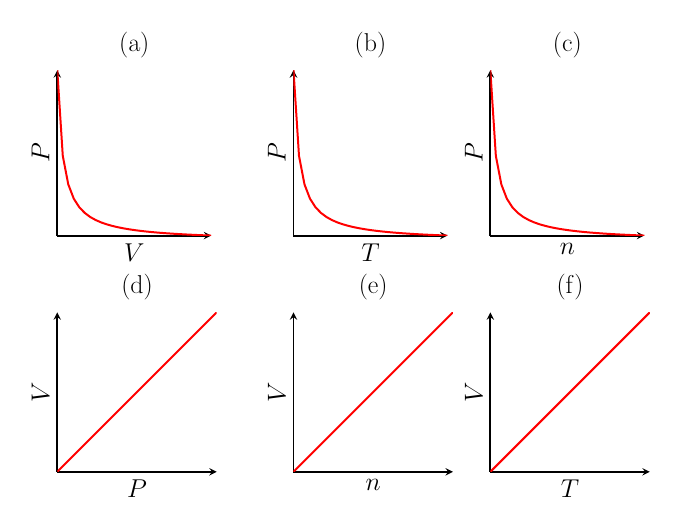
\begin{tikzpicture}[thick,scale=1.0, every node/.style={transform shape}]
 %%%%%%
 \begin{scope} [shift={(0.0,0.0)}, scale=0.45, transform shape]
\begin{axis}[xtick=\empty,ytick=\empty,ultra thick,y=1.5cm/3,title={\huge (a)},
    x=1.5cm,axis lines = left,yticklabels={,,},xticklabels={,,},
ylabel = {\huge $P$},	xlabel = {\huge $V$}
]
\addplot [ domain=0:3, samples=30, color=red]
{1/x};
\end{axis}
\end{scope}
 %%%%%%
  %%%%%%
 \begin{scope} [shift={(3.0,0.0)}, scale=0.45, transform shape]
\begin{axis}[xtick=\empty,ytick=\empty,ultra thick,y=1.5cm/3,title={\huge (b)},
    x=1.5cm,axis lines = left,yticklabels={,,},xticklabels={,,},
ylabel = {\huge $P$},	xlabel = {\huge $T$}
]
\addplot [ domain=0:3, samples=30, color=red]
{1/x};
\end{axis}
\end{scope}
 %%%%%%
  %%%%%%
 \begin{scope} [shift={(5.5,0.0)}, scale=0.45, transform shape]
\begin{axis}[xtick=\empty,ytick=\empty,ultra thick,y=1.5cm/3,title={\huge (c)},
    x=1.5cm,axis lines = left,yticklabels={,,},xticklabels={,,},
ylabel = {\huge $P$},	xlabel = {\huge $n$}
]
\addplot [ domain=0:3, samples=30, color=red]
{1/x};
\end{axis}
\end{scope}
 %%%%%%
   %%%%%%
 \begin{scope} [shift={(0.0,-3.0)}, scale=0.45, transform shape]
\begin{axis}[xtick=\empty,ytick=\empty,ultra thick,y=1.5cm,title={\huge (d)},
    x=1.5cm,axis lines = left,yticklabels={,,},xticklabels={,,},
ylabel = {\huge $V$},	xlabel = {\huge $P$}
]
\addplot [ domain=0:3, samples=30, color=red]
{x};
\end{axis}
\end{scope}
 %%%%%%
  %%%%%%
 \begin{scope} [shift={(3.0,-3.0)}, scale=0.45, transform shape]
\begin{axis}[xtick=\empty,ytick=\empty,ultra thick,y=1.5cm,title={\huge (e)},
    x=1.5cm,axis lines = left,yticklabels={,,},xticklabels={,,},
ylabel = {\huge $V$},	xlabel = {\huge $n$}
]
\addplot [ domain=0:3, samples=30, color=red]
{x};
\end{axis}
\end{scope}
 %%%%%%
  %%%%%%
 \begin{scope} [shift={(5.5,-3.0)}, scale=0.45, transform shape]
\begin{axis}[xtick=\empty,ytick=\empty,ultra thick,y=1.5cm,title={\huge (f)},
    x=1.5cm,axis lines = left,yticklabels={,,},xticklabels={,,},
ylabel = {\huge $V$},	xlabel = {\huge $T$}
]
\addplot [ domain=0:3, samples=30, color=red]
{x};
\end{axis}
\end{scope}
 %%%%%%
\end{tikzpicture}\end{center}



\end{question}
\begin{solution}
\begin{inparaenum}[(a)]	
\item  (a)
\item  (f)
\item (e)
\end{inparaenum} 
\hspace{0.1cm}\end{solution}\stepcounter{numA}%%%%%%%%%%%%

{\raggedright\textsc{\textbf{Change of Gas Properties }}\par}
%%%%%PROBLEM
\begin{question}[ID=\the\value{numA}]\SetQuestionProperties{section-title=\nameref{sec:units}}
A sample of a gas at 400K and 12 atm is cooled in the same container to 200K. Calculate the new pressure.
\end{question}
\begin{solution}
6 atm
\hspace{0.1cm}\end{solution}\stepcounter{numA}%%%%%%%%%%%%
%%%%%PROBLEM
\begin{question}[ID=\the\value{numA}]\SetQuestionProperties{section-title=\nameref{sec:units}}
In a storage area where the temperature has reached 300K, the pressure of oxygen gas in a 15 L steel cylinder is 1 atm. Calculate the volume if the pressure is reduced to 0.5 atm.
\end{question}
\begin{solution}
30L
\hspace{0.1cm}\end{solution}\stepcounter{numA}%%%%%%%%%%%%

%%%%%PROBLEM
\begin{question}[ID=\the\value{numA}]\SetQuestionProperties{section-title=\nameref{sec:units}}
A \ce{H2} sample has a volume of 5 L and a pressure of 1 atm. What is the new pressure if the volume is decreased to 2L with no change in temperature and the amount of gas. 
\end{question}
\begin{solution}
2.5L
\hspace{0.1cm}\end{solution}\stepcounter{numA}%%%%%%%%%%%%




%%%%%PROBLEM
\begin{question}[ID=\the\value{numA}]\SetQuestionProperties{section-title=\nameref{sec:units}}
A sample of Ne in a closed, expandable container, has a volume of 3L at 40$^\circ$C. Calculate the new volume if the container is cooled to 25$^\circ$C.
\end{question}
\begin{solution}
2.8 L
\hspace{0.1cm}\end{solution}\stepcounter{numA}%%%%%%%%%%%%
%%%%%PROBLEM
\begin{question}[ID=\the\value{numA}]\SetQuestionProperties{section-title=\nameref{sec:units}}
If the pressure of a gas increases, at fixed temperature and moles, its volume....
\end{question}
\begin{solution}
decreases
\hspace{0.1cm}\end{solution}\stepcounter{numA}%%%%%%%%%%%%
%%%%%PROBLEM
\begin{question}[ID=\the\value{numA}]\SetQuestionProperties{section-title=\nameref{sec:units}}
If the temperature of a gas increases, at fixed volume and moles, its pressure....
\end{question}
\begin{solution}
increases
\hspace{0.1cm}\end{solution}\stepcounter{numA}%%%%%%%%%%%%


{\raggedright\textsc{\textbf{Mixture of Gases and gas stoichiometry }}\par}
%%%%%PROBLEM
\begin{question}[ID=\the\value{numA}]\SetQuestionProperties{section-title=\nameref{sec:units}}
A tank contains Ne gas at 700 mmHg, Ar at 2 atm, and Kr at 700 torr. What is the total pressure of the mixture in atm?
\end{question}
\begin{solution}
1402torr
\hspace{0.1cm}\end{solution}\stepcounter{numA}%%%%%%%%%%%%
%%%%%PROBLEM
\begin{question}[ID=\the\value{numA}]\SetQuestionProperties{section-title=\nameref{sec:units}}
An anesthetic consist of a mixture of cyclopropane gas and oxygen gas. If the mixture has a total pressure of 2 atm and the partial pressure of cyclopropane is 0.5atm, what is the partial pressure of O2?
\end{question}
\begin{solution}
1.5atm
\hspace{0.1cm}\end{solution}\stepcounter{numA}%%%%%%%%%%%%



%%%%%PROBLEM
\begin{question}[ID=\the\value{numA}]\SetQuestionProperties{section-title=\nameref{sec:units}}
The atmospheric pressure on a hot day is 780 mmHg. Given that the air is made of 78\% of nitrogen and 22\% of oxygen, calculate the partial pressure of each gas in the air.
\end{question}
\begin{solution}
\ce{N2} 608 mmHg, \ce{O2} 171.6 mmHg
\hspace{0.1cm}\end{solution}\stepcounter{numA}%%%%%%%%%%%%
%%%%%PROBLEM
\begin{question}[ID=\the\value{numA}]\SetQuestionProperties{section-title=\nameref{sec:units}}
Phosphorus reacts with oxygen gas to produce tetraphosphorus decaoxide according to the following equation:
\begin{center}\ce{  P4(s)  + $\underset{\text{\large 2L}}{5\ce{O2(g)   }}$  -> $\underset{\text{\large x mol}}{\ce{P4O10(g)}}$  } \end{center}
Calculate the number of moles of phosphorus that react with 2L of oxygen at STP conditions.
\end{question}
\begin{solution}
0.017 mol
\hspace{0.1cm}\end{solution}\stepcounter{numA}%%%%%%%%%%%%

%%%%%PROBLEM
\begin{question}[ID=\the\value{numA}]\SetQuestionProperties{section-title=\nameref{sec:units}}
For the following reaction, calculate the unknown $x$ at STP conditions:
\begin{center}\ce{  C3H8(g)    + $\underset{\text{\large 5L}}{5\ce{O2(g)   }}$  -> $\underset{\text{\large x L}}{3\ce{CO2(g)}}$ + 4\ce{H2O_{(l)}}  } \end{center}
\end{question}
\begin{solution}
3L
\hspace{0.1cm}\end{solution}\stepcounter{numA}%%%%%%%%%%%%
%%%%%PROBLEM
\begin{question}[ID=\the\value{numA}]\SetQuestionProperties{section-title=\nameref{sec:units}}
For the following reaction, calculate the unknown $x$ at STP conditions:
\begin{center}\ce{  $\underset{\text{\large 3L}}{5\ce{C3H8(g)    }}$     + $\underset{\text{}}{5\ce{O2(g)   }}$  -> $\underset{\text{\large x L}}{3\ce{CO2(g)}}$ + 4\ce{H2O_{(l)}}  } \end{center}
\end{question}
\begin{solution}
1.8L
\hspace{0.1cm}\end{solution}\stepcounter{numA}%%%%%%%%%%%%
%%%%%PROBLEM
\begin{question}[ID=\the\value{numA}]\SetQuestionProperties{section-title=\nameref{sec:units}}
For the following reaction, calculate the unknown $x$ at STP conditions:
\begin{center}\ce{  $\underset{\text{\large 6moles}}{5\ce{C3H8(g)    }}$     + $\underset{\text{}}{5\ce{O2(g)   }}$  -> $\underset{\text{\large x L}}{3\ce{CO2(g)}}$ + 4\ce{H2O_{(l)}}  } \end{center}
\end{question}
\begin{solution}
80.64L
\hspace{0.1cm}\end{solution}\stepcounter{numA}%%%%%%%%%%%%




%%%%%PROBLEM
\begin{question}[ID=\the\value{numA}]\SetQuestionProperties{section-title=\nameref{sec:units}}
Consider the set up below with three different gases in three different closed containers at 300K. Assuming that the connecting tubes have zero volume, once the flasks are connected, calculate:
\begin{inparaenum}[(a)]	
\item  The partial pressure of each gas in the mixture
\item  The total gas pressure
\end{inparaenum} 

\begin{center}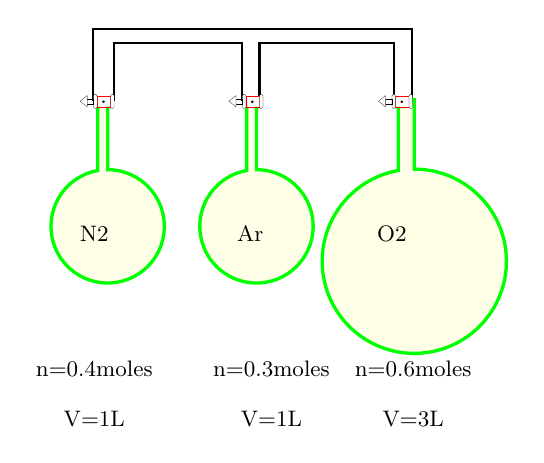
\begin{tikzpicture}[thick,scale=0.9, every node/.style={transform shape}]
\draw [black, fill=white,yshift=3.3cm, xshift=-.5] (0,0) -- ++ (0,1)-- ++ (4.5,0)   -- ++ (0,-1) -- ++ (-0.25,0) -- ++ (0,0.8)-- ++ (-1.9,0) -- ++ (0,-0.8) -- ++ (-0.25,0)-- ++ (0,0.8)-- ++ (-1.8,0)  -- ++ (0,-0.8) |- cycle ;
\draw [green, very thick,  fill=yellow!10, xshift=0.05cm,yshift=3.3cm]  (0,0)-- ++(0,-1) arc (100:450:0.8)   -- ++(0,1)  |- cycle ;
\draw [green, very thick,  fill=yellow!10, xshift=2.15cm,yshift=3.3cm]  (0,0)-- ++(0,-1) arc (100:450:0.8)   -- ++(0,1)  |- cycle ;
\draw [green, very thick,  fill=yellow!10, xshift=4.29cm,yshift=3.3cm]  (0,0)-- ++(0,-1) arc (100:450:1.3)   -- ++(0,1)  |- cycle ;
\begin{scope}[rotate=90,transform canvas={scale=.1},overlay,shift={(32cm,-2.3cm)}]
\draw [red, fill=white] (0,0) -- ++ (1.5,0)-- ++ (0,1.9)-- ++ (-1.5,0)   |- cycle ;
\draw[rounded corners=5pt, fill=white] (-0.25,1.9) rectangle ++(2,0.5);
\draw[rounded corners=5pt, fill=white] (-0.25,-.5) rectangle ++(2,0.5);
\draw (.7,1) node[circle, draw,fill=black]{};
\draw[xshift=9, yshift=1.4cm]  (0,1) rectangle ++(.8,1);
\draw [black, fill=white,yshift=3.3cm, xshift=-.5] (0,0) -- ++ (.8,1)-- ++ (.8,-1)    |- cycle ;
\end{scope}
\begin{scope}[rotate=90,transform canvas={scale=.1},overlay,shift={(32cm,-23.3cm)}]
\draw [red, fill=white] (0,0) -- ++ (1.5,0)-- ++ (0,1.9)-- ++ (-1.5,0)   |- cycle ;
\draw[rounded corners=5pt, fill=white] (-0.25,1.9) rectangle ++(2,0.5);
\draw[rounded corners=5pt, fill=white] (-0.25,-.5) rectangle ++(2,0.5);
\draw (.7,1) node[circle, draw,fill=black]{};
\draw[xshift=9, yshift=1.4cm]  (0,1) rectangle ++(.8,1);
\draw [black, fill=white,yshift=3.3cm, xshift=-.5] (0,0) -- ++ (.8,1)-- ++ (.8,-1)    |- cycle ;
\end{scope}
\begin{scope}[rotate=90,transform canvas={scale=.1},overlay,shift={(32cm,-44.4cm)}]
\draw [red, fill=white] (0,0) -- ++ (1.5,0)-- ++ (0,1.9)-- ++ (-1.5,0)   |- cycle ;
\draw[rounded corners=5pt, fill=white] (-0.25,1.9) rectangle ++(2,0.5);
\draw[rounded corners=5pt, fill=white] (-0.25,-.5) rectangle ++(2,0.5);
\draw (.7,1) node[circle, draw,fill=black]{};
\draw[xshift=9, yshift=1.4cm]  (0,1) rectangle ++(.8,1);
\draw [black, fill=white,yshift=3.3cm, xshift=-.5] (0,0) -- ++ (.8,1)-- ++ (.8,-1)    |- cycle ;
\end{scope}
\node [shift={(0,1.4)}, font=\small,scale=1] { \ce{N2} };
\node [shift={(2.2,1.4)}, font=\small,scale=1] { \ce{Ar} };
\node [shift={(4.2,1.4)}, font=\small,scale=1] { \ce{O2} };

\node [shift={(0,-0.5)}, font=\small,scale=1] {n=0.4moles};
\node [shift={(0,-1.2)}, font=\small,scale=1] {V=1L}; 
\node [shift={(2.5,-0.5)}, font=\small,scale=1] {n=0.3moles};
\node [shift={(2.5,-1.2)}, font=\small,scale=1] {V=1L}; 
\node [shift={(4.5,-.5)}, font=\small,scale=1] {n=0.6moles};
\node [shift={(4.5,-1.2)}, font=\small,scale=1] {V=3L};
\end{tikzpicture}\end{center}

\end{question}
\begin{solution}
\begin{inparaenum}[(a)]	
\item  $p_{\ce{N2}}$=1.97atm, $p_{\ce{Ar}}$=1.48atm,$p_{\ce{O2}}$=2.95atm
\item  6.40 atm
\end{inparaenum} 
\hspace{0.1cm}\end{solution}\stepcounter{numA}%%%%%%%%%%%%



%%%%%PROBLEM
\begin{question}[ID=\the\value{numA}]\SetQuestionProperties{section-title=\nameref{sec:units}}
Consider the set up presented below, where the connecting tubes have negligible volume. Calculate the partial pressure of each gas after the connection between the flasks is open.
\begin{center}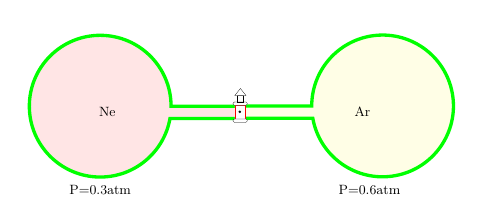
\begin{tikzpicture}[thick,scale=0.9, every node/.style={transform shape}]
\draw [green, very thick,  fill=red!10] (0,0) -- ++ (-1,0) arc (0:350:1.0) -- ++ (1,0)   |- cycle ;
\draw [green, very thick,  fill=yellow!10, yshift=.83cm]  (0,-1)-- ++(1,0) arc (190:540:1.0)  -- ++(-1,0)|- cycle ;
\begin{scope}[transform canvas={scale=.1},overlay,shift={(-1,-1.8)}]
\draw [red, fill=white] (0,0) -- ++ (1.5,0)-- ++ (0,1.9)-- ++ (-1.5,0)   |- cycle ;
\draw[rounded corners=5pt, fill=white] (-0.25,1.9) rectangle ++(2,0.5);
\draw[rounded corners=5pt, fill=white] (-0.25,-.5) rectangle ++(2,0.5);
\draw (.7,1) node[circle, draw,fill=black]{};
\draw[xshift=9, yshift=1.4cm]  (0,1) rectangle ++(.8,1);
\draw [black, fill=white,yshift=3.3cm, xshift=-.5] (0,0) -- ++ (.8,1)-- ++ (.8,-1)    |- cycle ;
\node [shift={(-19,-10)}, font=\small,scale=6] {P=0.3atm};
\node [shift={(-19,-14)}, font=\small,scale=6] {V=1L}; 
\node [shift={(19,-10)}, font=\small,scale=6] {P=0.6atm};
\node [shift={(19,-14)}, font=\small,scale=6] {V=1L}; 
\node [shift={(-18,1)}, font=\small,scale=6] {\ce{Ne}}; 
\node [shift={(18,1)}, font=\small,scale=6] {\ce{Ar}}; 
\end{scope}
\end{tikzpicture}\end{center}
\end{question}
\begin{solution}
\item  $p_{\ce{Ne}}$=0.15atm, $p_{\ce{Ar}}$=0.3atm

\hspace{0.1cm}\end{solution}\stepcounter{numA}%%%%%%%%%%%%






{\raggedright\textsc{\textbf{Real gases and the kinetic molecular theory of gases }}\par}

%%%%%PROBLEM
\begin{question}[ID=\the\value{numA}]\SetQuestionProperties{section-title=\nameref{sec:units}}
What is the pressure in atm of 1 mol of He at 600K in a 1L container: 
\begin{inparaenum}[(a)]	
\item  Using the ideal gas law
\item  Using the real gas law given $a=$ 0.0342$\text{atm}\cdot \text{L}^2/\text{mol}^{2}$ and $b=$ 0.0237$\text{L/mol}$
\end{inparaenum} 
\end{question}
\begin{solution}
\begin{inparaenum}[(a)]	
\item  49.2 atm
\item  50.36 atm
\end{inparaenum} 
\hspace{0.1cm}\end{solution}\stepcounter{numA}%%%%%%%%%%%%

%%%%%PROBLEM
\begin{question}[ID=\the\value{numA}]\SetQuestionProperties{section-title=\nameref{sec:units}}
Calculate the pressure $p$ in atm exerted by 2 moles of methane (\ce{CH4}) in a 0.5L container at 300K. 
\begin{inparaenum}[(a)]	
\item  Using the ideal gas law $p^{ideal}$
\item  Using the real gas law $p^{real}$, given $a=$ 2.283 $\text{atm}\cdot \text{L}^2/\text{mol}^{2}$ and $b=$ 0.04278$\text{L/mol}$
\item Calculate the percent error in the ideal gas law using $\abs{p^{ideal}-p^{real}}/p^{real}\times 100$.
\end{inparaenum} 
\end{question}
\begin{solution}
\begin{inparaenum}[(a)]	
\item   98.4 atm
\item   82.1 atm
\item 17\%
\end{inparaenum} 
\hspace{0.1cm}\end{solution}\stepcounter{numA}%%%%%%%%%%%%


%%%%%PROBLEM
\begin{question}[ID=\the\value{numA}]\SetQuestionProperties{section-title=\nameref{sec:units}}
Use the Van der walls constant $a$ to compare which of the gases exhibit stronger intermolecular interactions between its particles for the following pair of gases:
\begin{inparaenum}[(a)]	
\item  Ar or Ne
\item  CO or NO
\end{inparaenum} 
\end{question}
\begin{solution}
\begin{inparaenum}[(a)]	
\item   Ar
\item   CO
\end{inparaenum} 
\hspace{0.1cm}\end{solution}\stepcounter{numA}%%%%%%%%%%%%


%%%%%PROBLEM
\begin{question}[ID=\the\value{numA}]\SetQuestionProperties{section-title=\nameref{sec:units}}
Without consulting the values of the Van der walls constant $b$ indicate which of the gases of  the following pair would exhibit a larger $b$ value:
\begin{inparaenum}[(a)]	
\item  \ce{C2H6} or \ce{CH4}
\item  \ce{H2} or \ce{CH4}
\end{inparaenum} 
\end{question}
\begin{solution}
\begin{inparaenum}[(a)]	
\item   \ce{C2H6}
\item   \ce{CH4}
\end{inparaenum} 
\hspace{0.1cm}\end{solution}\stepcounter{numA}%%%%%%%%%%%%


%%%%%PROBLEM
\begin{question}[ID=\the\value{numA}]\SetQuestionProperties{section-title=\nameref{sec:units}}
What is the rms speed of \ce{O2} at STP?.
\end{question}
\begin{solution}
481.9 m/s
\hspace{0.1cm}\end{solution}\stepcounter{numA}%%%%%%%%%%%%
%%%%%PROBLEM
\begin{question}[ID=\the\value{numA}]\SetQuestionProperties{section-title=\nameref{sec:units}}
Order the following molecules in increasing order of root-mean square velocity: Ne, \ce{CO2}, \ce{H2O}, \ce{CH4}.
\end{question}
\begin{solution}
$v_{rms}^{\ce{Ne}}$ $<$ $v_{rms}^{\ce{CH4}}$ $<$ $v_{rms}^{\ce{H2O}}$$<$ $v_{rms}^{\ce{CO2}}$
\hspace{0.1cm}\end{solution}\stepcounter{numA}%%%%%%%%%%%%



%%%%%PROBLEM
\begin{question}[ID=\the\value{numA}]\SetQuestionProperties{section-title=\nameref{sec:units}}
The kinetic molecular theory of gases assumes that:
\noindent
  \begin{enumerate} [topsep=0pt, partopsep=1pt, label=(\alph*), leftmargin=0.5cm]	
\item gas particles interact with each other
\item gas particles have large sizes
\item particles move slowly
\item gas particles move randomly
\end{enumerate}
\end{question}
\begin{solution}
gas particles move randomly
\hspace{0.1cm}\end{solution}\stepcounter{numA}%%%%%%%%


%%%%%PROBLEM
\begin{question}[ID=\the\value{numA}]\SetQuestionProperties{section-title=\nameref{sec:units}}
For the velocity distribution curved below:
\begin{inparaenum}[(a)]	
\item  The plots represent the distribution of velocity of two gases \ce{Ne } or \ce{Ar} at STP conditions in a fixed volume. What line represents each gas?
\item  The plots represent the distribution of velocity of a gas at two different temperatures 300K and 500K at fixed pressure and volume conditions. What line represents each each temperature?
\end{inparaenum} 


\begin{center}\begin{tikzpicture}[thick,scale=0.5, every node/.style={transform shape}]
\begin{scope}[xshift = 0cm]
\pgfkeys{/pgfplots/linelabel/.style args={#1:#2:#3}{name path global=labelpath,execute at end plot={
\path [name path global = labelpositionline]
(rel axis cs:#1,0) --
(rel axis cs:#1,1);
\draw [help lines,text=black,inner sep=0pt,name intersections={of=labelpath and labelpositionline}] (intersection-1) -- +(#2) node [label={#3}] {};},
}}
\pgfplotsset{ compat  = 1.13,samples = 100,}
\def\kB{1.3806488e-23}% boltzmann constant
\def\temperature{300}% room temperature
\def\Beta{1/(\kB*\temperature)}
\def\amu{1.660538921e-27}% atomar mass unit in kg
\def\mass{28*\amu}
\def\mB{\mass*\Beta}
\begin{axis}[
  axis lines = left,
  domain     = 0:1500,
  xlabel     = Molecular velocity (m/s),
  ylabel     = Number of molecules,
  xtick      = \empty,
%xmax = 1500,
  ytick      = \empty,
  clip       = false,
]
  \addplot[black, linelabel=0.3:{.6cm,.6cm}: {[black]right:(a)}]		 {sqrt(2/pi)*(\mB)^(3/2)*x^2*exp(-.5*\mB*x^2)};
  \def\temperature{300}% room temperature
\def\Beta{1/(\kB*\temperature)}
\def\amu{1.660538921e-27}% atomar mass unit in kg
\def\mass{70*\amu}
\def\mB{\mass*\Beta}
   \addplot[red, linelabel=0.2:{.6cm,.6cm}: {[red]right:(b)}]{sqrt(2/pi)*(\mB)^(3/2)*x^2*exp(-.5*\mB*x^2)};
\end{axis}
\end{scope} 
\end{tikzpicture}
\end{center}
\end{question}
\begin{solution}
\begin{inparaenum}[(a)]	
\item  b is \ce{Ne } and a is \ce{Ar} 
\item  b is 500K and a is 300K 
\end{inparaenum} \hspace{0.1cm}\end{solution}\stepcounter{numA}%%%%%%%%%%%%


\end{multicols*}
\newpage
\begin{answersenvironment}
\begin{minipage}[c]{1\textwidth}
\begin{localsize}{10}
{\Large \bf Answers}
\SetupExSheets{
  headings = inline-nr , % numbered and inline
  counter-format = qu) , % numbers 1) 2) ... 
}
%\printsolutions 
\printsolutions[byID={1,3,5,7,9,11,13,15,17,19,21,23,25, 27, 29, 31, 33, 35 }]
\end{localsize}
\end{minipage}\end{answersenvironment}
\end{document}




%\documentclass[main.tex]{subfiles}
%\begin{document}\newpage
%\setdoublesep{0.35700 em}  % 'Bond Spacing'
%\setatomsep{1.78500 em}    % 'Fixed Length'
%\setbondoffset{0.18265 em} % 'Margin Width'
%\newcommand{\bondwidth}{0.06642 em} % 'Line Width'
%\setbondstyle{line width = \bondwidth}
%\newgeometry{left=0.8in,right=0.8in, top=2.5cm,bottom=2cm}
%\fancyhfoffset[E,O]{0pt}
%\setlength{\columnsep}{30pt}
%\begin{conclusion}
%\end{conclusion}
%\setstretch{0.3}
%\begin{multicols*}{2}

%





%
%
%
%
%
%

%
%\restoregeometry
%\end{enumerate}
%\end{multicols*}
%\pagecolor{green!10}\afterpage{\nopagecolor}\newpage
%\end{document}